\section{Motivation}
Modern day technology has developed under incredible speed in recent decade and the computing power growth rate is truly phenomenal and lasting impact can be felt and benefit us in many ways. It is important to realise the worldwide effect on environment by the increase in consumption of power by these technology advancements.

According to~\cite{pickavet2008worldwide}, the power consumption growth rates of PCs are about 7.5\% per year. Data Centres and network play much larger role as they both have power consumption rate of 12\% each. This considerable growth is due to increasing data to be accessed, stored and processed. The constant expansion of energy consumption leads to increase in carbon emissions. \(CO_2\) emissions from ICT (Information and communications technology) are increasing at a rate of 6\% per year, at such rate by 2020 it will account to 12\% of worldwide emissions ~\cite{rong2016optimizing}.

\begin{figure}[ht]
	\centering
	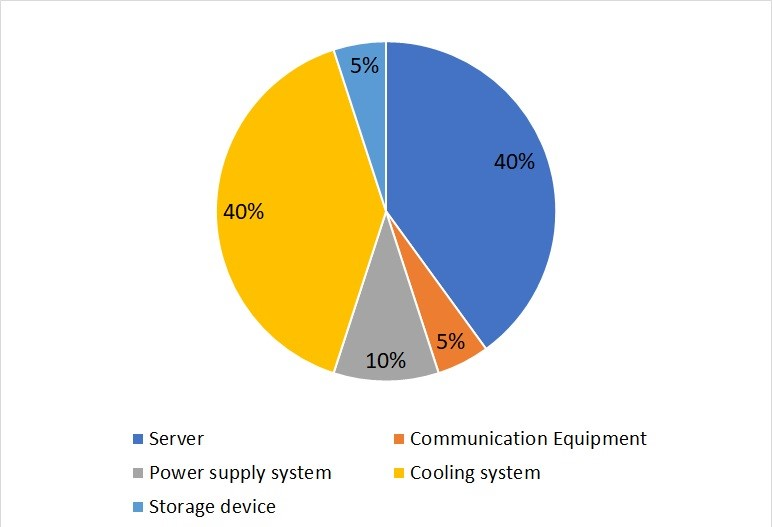
\includegraphics[width=300pt]{energypiechart}
	\caption{\label{fig:energypie} Energy consumption distribution of data centers.}
\end{figure}

The major roles of power consumption by a data ware house is played by the servers and the cooling system which is used to cool down the server physical parts. The figure~\ref{fig:energypie}, shows that both the servers and the cooling systems account to 80\% of the total consumption with both accounting for 40\% each~\cite{rong2016optimizing}. Making power and energy one of the key challenges in system and software designs. In order to improve processor's performance while limiting power consumption, designers have increasingly utilized dynamic hardware adaptions. But to guide to these hardware adaptions it is necessary to measure the power of systems accurately. Such adaptations can reduce power consumption and chip temperature by reducing the amount of available performance. Temperature sensors are slow in reponse due to the thermal inertial of the micro processor. Relying on them would give slow response and detection of temperature changes. Many demonstrations have been done to show that performance counter / performance events are effective proxies of power measurement \cite{bellosa2000benefits}.

The study of the relations between different performance counters and energy consumption has become crucial. The existence and analysis of relations can enable minimization of power consumption leading to less heat generation from the CPU. This decrease in temperature can further reduce the usage of cooling system. This all in turn leads to cost minimization and a step towards eco-friendly environment.

Thus, discovery of the functional relation between the power consumption and the performance events (PMCs) of system, will enable the ability to adjust, and predict the energy consumption for certain computations.

\section{Aims}

The project aims to create a piece of software that will help understanding and finding relations between energy consumption and performance counters. The software must aim to be extensible, easy to use and performant. It should be able to perform analysis like regression and clustering on the data. These actions will help in showcasing the relationship of various parameters and the output. In this case, the parameters are the performance events and output is the energy consumption by the systems. Following are the objectives that are attempted to be accomplished.

\subsection{Existence of functional relation}

Datasets are mostly pair of multiple inputs and a single output. And the possibility of the existence of a relation is what have to be found. Is it possible to define the data in a form of function? Question like this is one of the aims. Defining the data in a form of function can be thought of as explaining the dataset in a form of a formula which can combine various parts of the input parameters and match the output. It is quite impossible to tell that whether a function definetly exists as the data is always a subset of the population and there are number of records which are either not in the dataset or it is not know. But, regardless it can definitely explain the non-existence of a formula by finding a pair of input parameters and outputs that violate the definition of a function.

The pair which violates the definition of a function must be looked at as there is high probability of that data set record being corrupt or if not it can actually act as a contradictiona and explain the non existence. If this outlier is in fact corrupt, this process can be used for data cleanups as well.

\subsection{Analysis of functional relation}

Once, it is not possible to prove functional non existence in the dataset. The dataset must be analysed. In order to better understand the the functional relation of the parameters with the output. The analysis of the relation explains the contribution of a parameter to the result. It gives better understanding about the correlation between two quantities. Does high page faults correlates to high energy consumption? Questions like this is what the analysis of change in parameters with their corresponding change in output answers. This can also be thought of an explaination of the resultant parameter.

In other words, understanding the correlation is the other aim. Once it is know that there is high correlation. Further investigation can be done in order to find the form of the relation.

\section{Approach}

For each of the aims, two approaches have been employed. Both the approaches tries to achieve the same conclusions but with different methodology.

The experimental data sets provided has the following format:

\(E_1,\ x_{11},\ x_{12},\ x_{13} \ldots x_{1k}\)\\
\(E_1,\ x_{21},\ x_{22},\ x_{23} \ldots x_{2k}\)\\
\ldots \\
\(E_n,\ x_{n1},\ x_{n2},\ x_{n3} \ldots x_{nk}\)

where \(k\) is the number of parameters (performance events), \(n\) is the number of records in the dataset.
\(E_i\) is the experimentally obtained dynamic energy consumption and \(x_{ij}\) are the experimentally obtained performance events (PMCs).

\subsection{Existence of functional relation}

The main objective here is to find the nonexistence of functional relationship. In other words, it means proving that the dataset cannot be explained in terms of a function/formula.

First approach here is to find two performance events tuples \((x_{i1},\ x_{i2},\ x_{i3} \ldots x_{ik})\) and \\ \((x_{j1},\ x_{j2},\ x_{j3} \ldots x_{jk})\) that are equal within some tolerance, but their corresponding \(E_i\) and \(E_j\) dynamic energy consumption are different. Existence of such a tuple in database will lead us to prove the non-existence of a functional relationship.

It is infact easier to find two equal records by ordering the dataset by their parameters and going through the entire dataset once to find equal records and comparing their dynamic energy consumption. The order of complexity of such is \(O(N \log(N))\) which is the complexity of sorting as that is the only heavy duty task involved. But it gets complicated when tolerance comes into play. Likewise, task at hand is to find similar records rather than equal records. The project employs 2 methods to measure the similarity between the two data records.

First approach:

The data records are imagined as data points in \(k-space\) as we have \(k\) number of parameters. Then the whole space is divided into small \(k-dimension cubes\) with dimensions \((t_1, t_2, \ldots t_k)\) where \(t_i\) is the tolerance of each parameter. The data points are then put in their respective cubes. And each cube is then analysed to see whether the output of the data points are similar to each other as well.

Second approach:

The data points in \(k-space\) are similar if the euclidean distance between them is less than the \(t\) provided, where \(t\) is the total/max tolerance. Data points which are infact found to be close to each other, their output is compared to see if they are similar to each other.

\subsection{Analysis of functional relation}

Many different type of relations can exists between two variables. But, since correlation betweent the variables is the objective been set. A more general trend of the dynamic energy consumption with the performance events is analysed. Many researches have been done that successfully using linear models, to understand the relation between energy consumption and performance events.\cite{o2017survey} The preference given to linear models is due to the trickle down effect of the performance events.\cite{bircher2007complete} Hence, Linear regression is used to analyse the relationship.

Linear regression is done with 2 variables but there are \(k\) variables relation to energy consumption making it hard to understand the nature. Multiple linear regression tries to find the best fit to the data. Best fit to the data hinders the tolerance factor in the dataset and also undermines the actual relation. As multiple regression tries to find the best fit and is interested in predicting the output variable. Hence to analyse one of the variable, the data point must be grouped such that their other \(k-1\) variables are constant. Each cluster is then visited and linear regression is performed. Two approaches are employed to cluster which are similar to finding similar records in finding the existence of the relation.

First approach:

Data points are clustered by putting the data points in the respective \(k-1\) dimension cube. Forming a cluster with almost similar \(k-1\) variables.

Second approach:

Euclidean distance is used to isolate similar \(k-1 variables\). A \(k-1\) dimension sphere can be imagined for simplicity with its radius being the total/max tolerance.

In both approaches, linear regression is performed on the cluster with the variable which was not used in clustering and the output variable which corresponds to the dynamic energy consumption.

\section{Structure of report}

In this report, the motivation behind the project and brief description of the approaches that will be undertaken to reach the objective are seen already.

This Introductory chapter is followed by Background research, design aspects of the software, implementation of the software, testing and evaluation of the tool followed by the conclusion and the future works.

Background research explains about performance events and how do they influence energy consumption by the system. It also explains the approaches in detail mentioned above and analyses their complexity and how they can be optimised.

Following Background research, design and implementation of the software is deep dig into as we want an extensible, performant tool. Testing and evaluation of the software is explained. How the software is tested and its evaluation on its performance. The report ends with conclusions and future works that shows how the project can be extended and applied to various other domains.